\documentclass{amsart}
\usepackage[scaled]{helvet}
\renewcommand*\familydefault{\sfdefault} % These two commands set the base font of the document to sans serif

\usepackage{mathrsfs} %I don't know what this package is, but I was scared to delete is
\usepackage{amssymb} %Standard packages
\usepackage{amsmath}
\usepackage{amsthm}
\usepackage{sansmath} %This makes the math symbols match sans serif
\usepackage{color}
\usepackage{hyperref} %Makes hyperlinked Theorem, Figure, and Citation links
\usepackage{epsfig}
\usepackage{graphicx}
\usepackage{lipsum}  % Lorem Ipsum placeholder text for the outline.
\input xy
\usepackage{subfig}
\graphicspath{ {./Images/} }
\xyoption{all}

\usepackage{fancyhdr} %Package that allows for neat headers
\pagestyle{fancy}
\fancyhead[LE]{{\sc Proc. Stockton Math. Sem.}} %Header on the left of even numbered pages
\fancyhead[LO]{\textit{\leftmark}} %Header on the left of odd numbered pages
\fancyhead[RE]{\textit{\leftmark}} %Header on the right of even numbered pages
\fancyhead[RO]{\shorttitle} %Header on the right of odd numbered pages
\cfoot{\thepage} %Footer commands
% End of pile of commands that makes the header!

% FIRST PAGE NUMBER
\setcounter{page}{0}                  %%%%%%%
\setlength{\textwidth}{4.4in}          %%%%%%%
\setlength{\textheight}{7.0in}         %%%%%%%
\setlength{\evensidemargin}{1in}       %%%%%%%
\setlength{\oddsidemargin}{1in}        %%%%%%%
\setlength{\topmargin}{.8in}

\newtheorem{theorem}{Theorem}[section]
\newtheorem{lemma}[theorem]{Lemma}
\newtheorem{proposition}[theorem]{Proposition}
\theoremstyle{definition}
\newtheorem{definition}[theorem]{Definition}
%\newtheorem*{maintheorem}{Theorem \ref{thm:main}}
\newtheorem{remark}[theorem]{Remark}
\numberwithin{equation}{section}

%%%% HERE YOU CAN DEFINE YOUR FAVORITE SHORTCUT COMMANDS:
%
    % VECTORES (boldface)
    \def\ve#1{{\bf #1}}
    % NORMS OF THESE BEASTS:
    \def\norm#1{\| {\bf #1} \|}
    % JUST NORMS
    \def\norma#1{\| { #1} \|}
    % VECTORES CON FLECHITA: (december 2003)
    \def\vector#1{\overrightarrow{\strut{#1}}}
    % Rn
    \def\rn{{\Bbb R}^n}
    % Blackboard R
    \def\r{{\Bbb R}}
    % ABS value
    \def\abs#1{\vert \, {#1} \, \vert}

    % dS/dt, dI/dt, dR/dt
    \newcommand{\dS}{\frac{dS}{dt}}
    \newcommand{\dI}{\frac{dI}{dt}}
    \newcommand{\dR}{\frac{dR}{dt}}

%%%%%%%%%%%%%%%%%%%%%%%%%%%%%%%%%%%%%%%%%%

\begin{document}

\begin{sansmath}

\begin{center}
\begin{picture}(256,56)
\put(63,37){\textbf{Proceedings of the Stockton}}
% \put(55,23){\textbf{University Mathematics Seminar}}
\put(79,23){\textbf{Mathematics Seminar}}
%\put(85,11){\tiny{Presented on [date of the presentation]}}
%\put(0,0){\framebox(255,54){}}
%\put(2,2){\framebox(251,50){}}
%\put(8,10){
\includegraphics[scale = .55]{Stockton.png}}
%\put(210,10){
\includegraphics[scale = .5]{Sigma.png}}
\end{picture}
\end{center}

\title[Running Title (shorter)]
{SIR Modeling and Covid}

\author{Steven Blythe}
\email{StevenBlytheSU@gmail.com}


\keywords{}

\begin{abstract}
ABSTRACT HERE

\end{abstract}

\maketitle

\section{Introduction}

What is Differential Equations and why do we use it to model infectious diseases? It is important to note that the goal of mathematical models are not to create a perfect representation of an event occurring in the real world. Instead, mathematical models are a mere representation of an event with the goal to help understand an aspect of the event. % 2

While we may use mathematical models, we must take note that the real world has many variables that complicates our representation. For example, we might make a model for the amount of crop yield in a given year based on crop data. However, we may say blueberries tend to bloom over the summer so we should expect a higher yield over the summer, real-world factors such as droughts, demand fluctuation, and ongoing diseases may lower crop yield in a given year.

When we build models, we should look to compare our model with data from the real world. If our model accurately describes what we are representing, then we have created a tool to assist us in predicting a system. Otherwise, if our model is wrong, we should study and pay close attention to our model to improve our knowledge for our assumption.

\section{Model Building}

Think to yourself. How do you think you might model population growth? If we have a population of $100$ in a given year, we might first consider adding a fraction of our population back into the total population. As the population grows, the fraction we add back in also grows. Our model may only have a few factors considered, but our model is a good basis for what we are looking for. Our model suggests the rate of growth of our population is proportional to the population itself. Using this assumption, we can derive a working model with variables.

We established a population for our model, a population of $100$, in our first model for population growth. Instead of using $100$, we can use variable $P$ to represent our population size. We also represented our population growth in terms of a fraction, or $k$. Here, we have a simple model to represent change from one instance. However, how should we find our population after many days? Here, we can use $t$ to represent years and $P(t)$ will represent the quantity of our population.

If we want to consider a model where we can find the rate of change of our population $P$, we might want to find $\frac{dP}{dt}$. Now, from our assumption, we are looking for a model where we can measure the rate of growth for a given population. We know this rate of growth is proportional to our population. Here, we want to look for the following differentual equation:

\[ \frac{dP}{dt} = kP \]

Here, we created a differential equation. Our differential equation is a first-order equation since we are only considering the first derivative of our dependent variable.

\section{Finding Meaning in our Models}

For the model we created, we know our model will predict our population after a given amount of time. Our model always assume our population will grow at a rate $k$. What would it mean if $\frac{dP}{dt} = 0$? Since our rate of growth is positive, that means our population $P$ must have began at $0$. Here, we can represent our equation as:

\[ \frac{dP}{dt} = k(0)\]

For all our $t$, $P(t) = 0$. Since $k$ is a positive constant, we can expect to have a population of $0$ if our population begins at $0$ at $t = 0$, or $t_0$. We can represent our initial population, or initial condition, as $P(t_0)$.

Can we expect our differential equation to be negative at some point? Since we are looking at a population, we only want to consider $kP \geq 0$, which would never 'grow' into a negative population.

Now, can we graph our equation right now? Not yet. If we graph $kP$, we only have a linear graph. Should our growth, which is proportional to our current population, produce a linear graph? If our growth is $10\%$ and our initial population is $100$, we may expect an increase of roughly $10$ people in one time step. If we move another time step, should we expect the same increase of $10$ or should we expect an increase of $11$? To find the equation we can use to predict our growth, we must solve our differential equation. If we solve our differential equation, our solution is as follows:

\[ P(t) = ce^{kt} \]

% Perhaps perform the solution?

This is the general solution for our system. Remember, $k$ is our rate of growth and $t$ represents time. Note that we also added $c$ to our equation. The constant $c$ came from an integration we performed to find our solution. To find $c$, we use our initial condition $P(t_0)$. If $P(t_0)$ is $10$, then we have:

\begin{align*}
  P(t_0) & = ce^{k(0)}\\
  10 & = c\\
  P(t) & = 10e^{kt}
\end{align*}

Here, we a specific solution for our initial condition, $P(t_0) = 10$. We can plot the specific solution to predict our population growth. Now, let us consider a few initial conditions for our starting population. Remember, population should be non-negative. Let us let $P(t_0)$ be $0$ first.
\begin{center}
  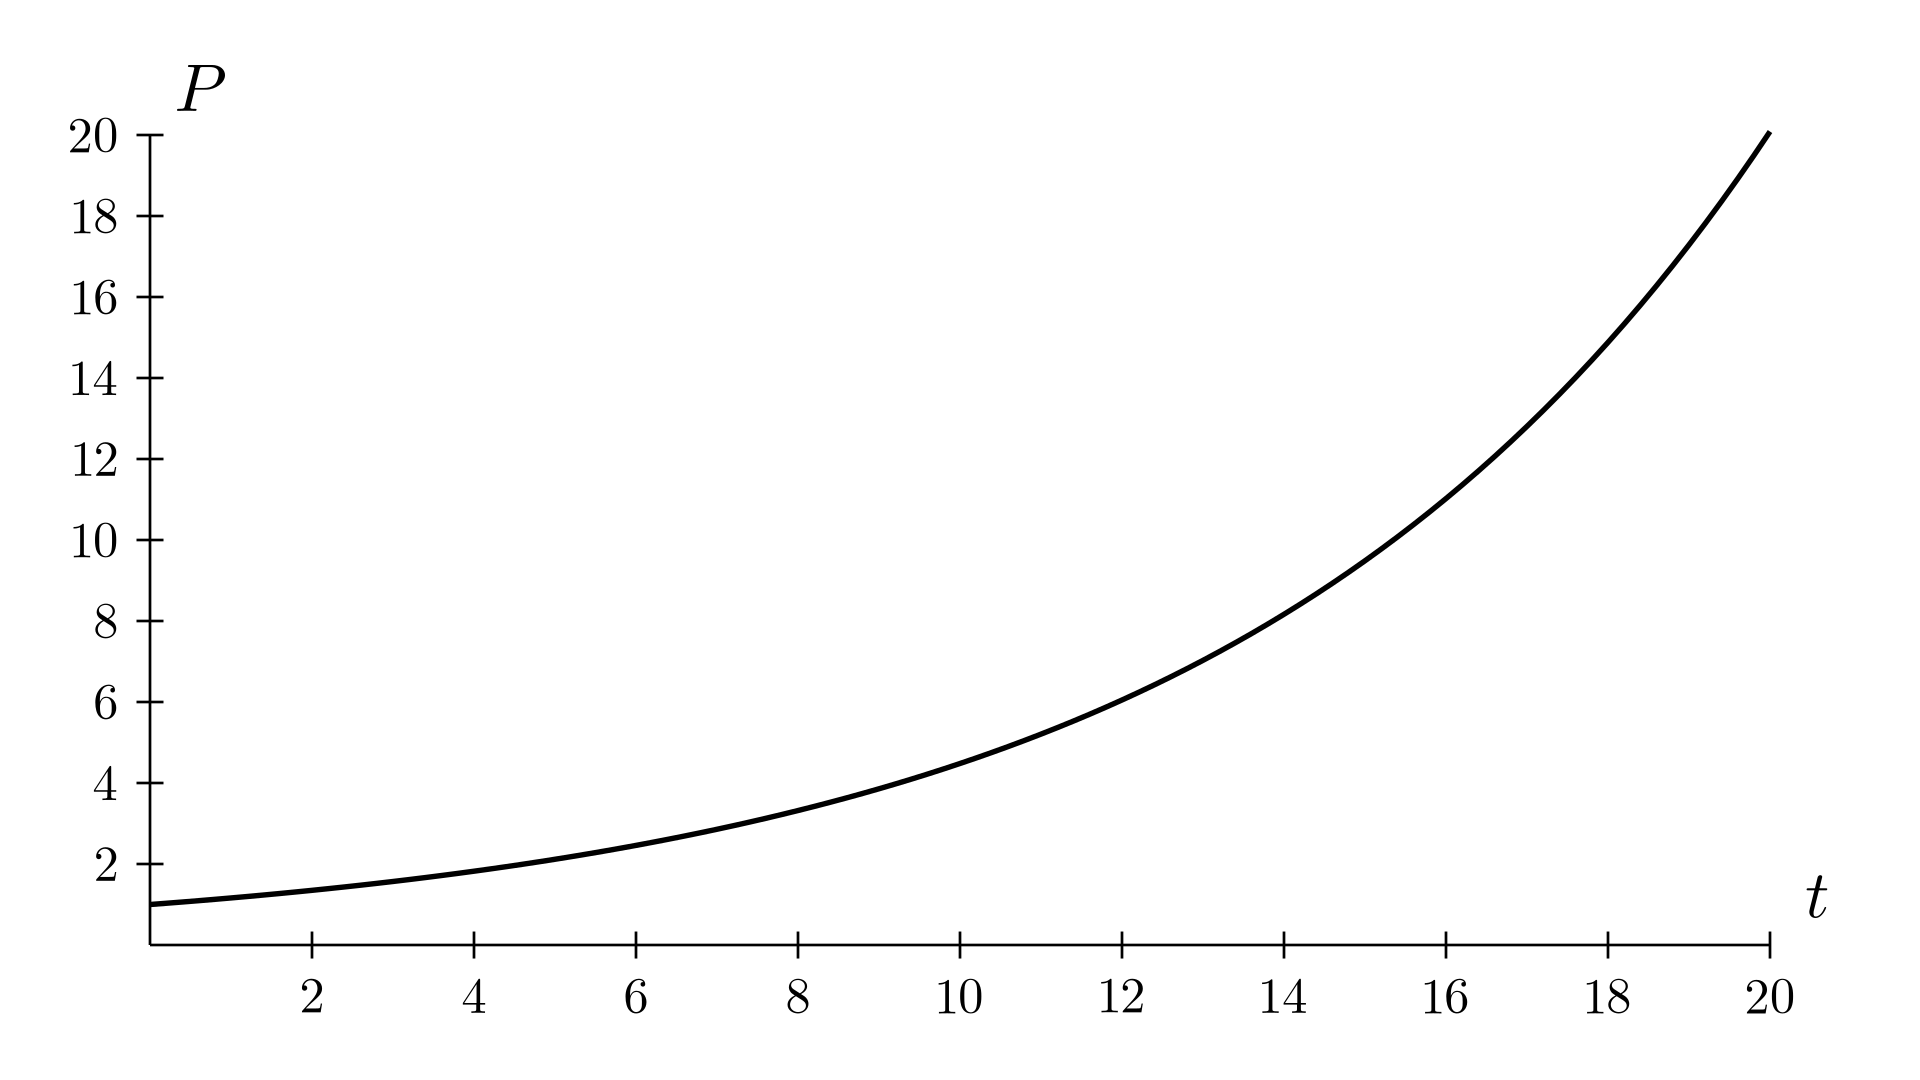
\includegraphics[width=10cm]{ExponentialGrowthSingle}
\end{center}
% Graph here | c = 0,

Looking at the graph, we can see our population is always $0$ for all of $t$. Now, let us consider a few other examples, such as $P(t_0) = 0, 0.5, 1, 1.5, \ldots, 10$.

% Graph here | c = 100, 200, 500
\begin{center}
  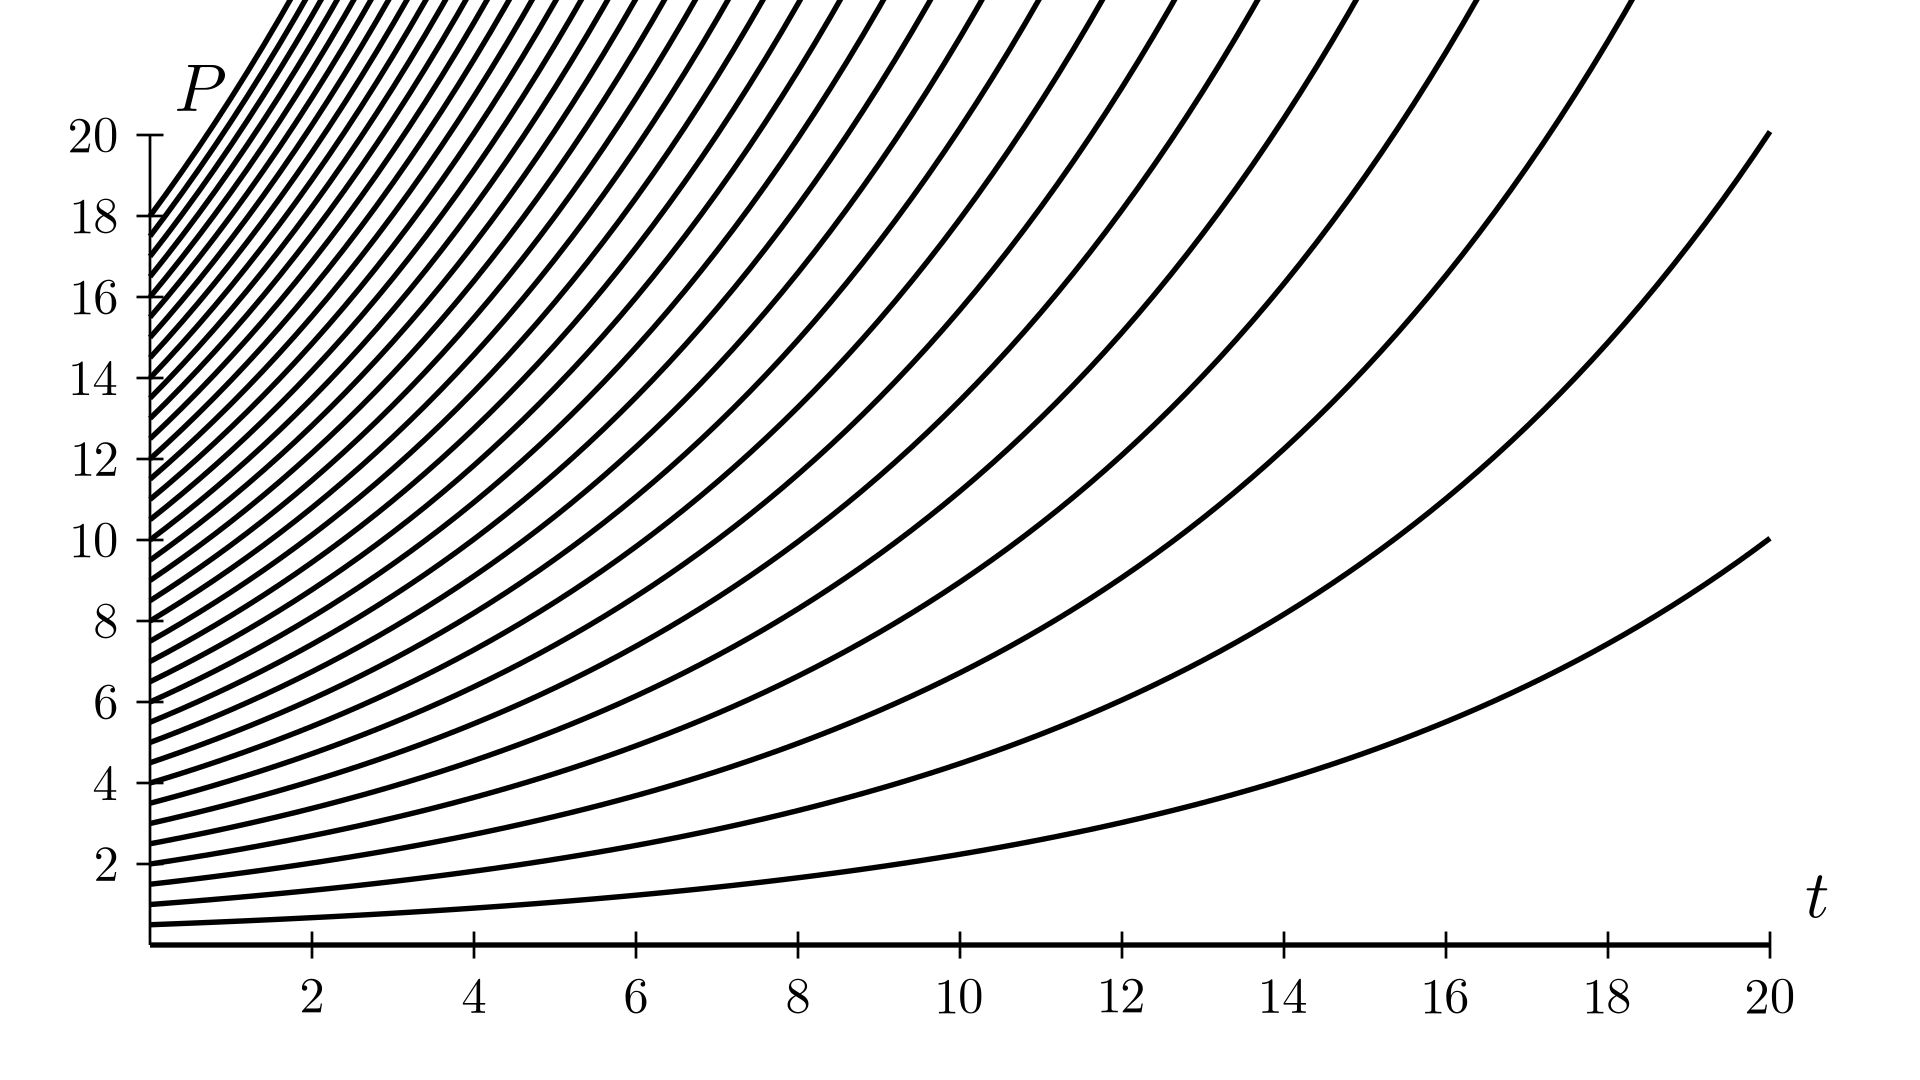
\includegraphics[width=10cm]{ExponentialGrowGroup}
\end{center}

\section{Logistic Population Model}

Looking at the graphs in the previous section, should we expect our model to work in the real world? Not always. If we're modeling the population of rabbits in an area, we may expect an initial growth. However, as time goes on, there will eventually be not enough resources for all the rabbits in an area. Now, we want a model where we can predict a growth while under a threshold but a decay above a threshold. Let us look at our original equation for growth:

\[ \frac{dP}{dt} = kP \]

Here, let us consider a threshold for our equation, $N$. Let us consider a few cases surrounding $N$:

\begin{enumerate}
  \item If $P < N$, let population grow: $\frac{dP}{dt} \approx kP$
  \item If $P = N$, let our population growth become stagnant.
  \item If $P > N$, let population decrease: $\frac{dP}{dt} < 0$
\end{enumerate}

Here, we can see our population size and threshold are related in some way. If $P < N$, we should expect a positive number, whereas if $P > N$, we should expect a negative number. One way we can represent this is with the following:

\[ (1 - \frac{P}{N} )\]

Here, we can plug our new expression into our original equation.

\[ \frac{dP}{dt} = kP \Big(1 - \frac{P}{N} \Big) \]

If we go ahead and solve for the general solution, we can expect to find:

\begin{align*}
  P(t) & = \frac{N}{1 - ce^{-kt}}
\end{align*}

Here, we can use our general solution to help us plot different particular solutions. Note that $k$ is our rate of growth, $t$ is time, $N$ is our carrying capacity, and $c$ is our constant from our integration. When we set $P(0)$, we can find our initial condition.

What can we expect to find with our graph? Will our initial condition always grow to infinity, or can we expect to experience a decay after a period of growth? Here, let us plot a few particular solutions. % For N, k

\begin{center}
  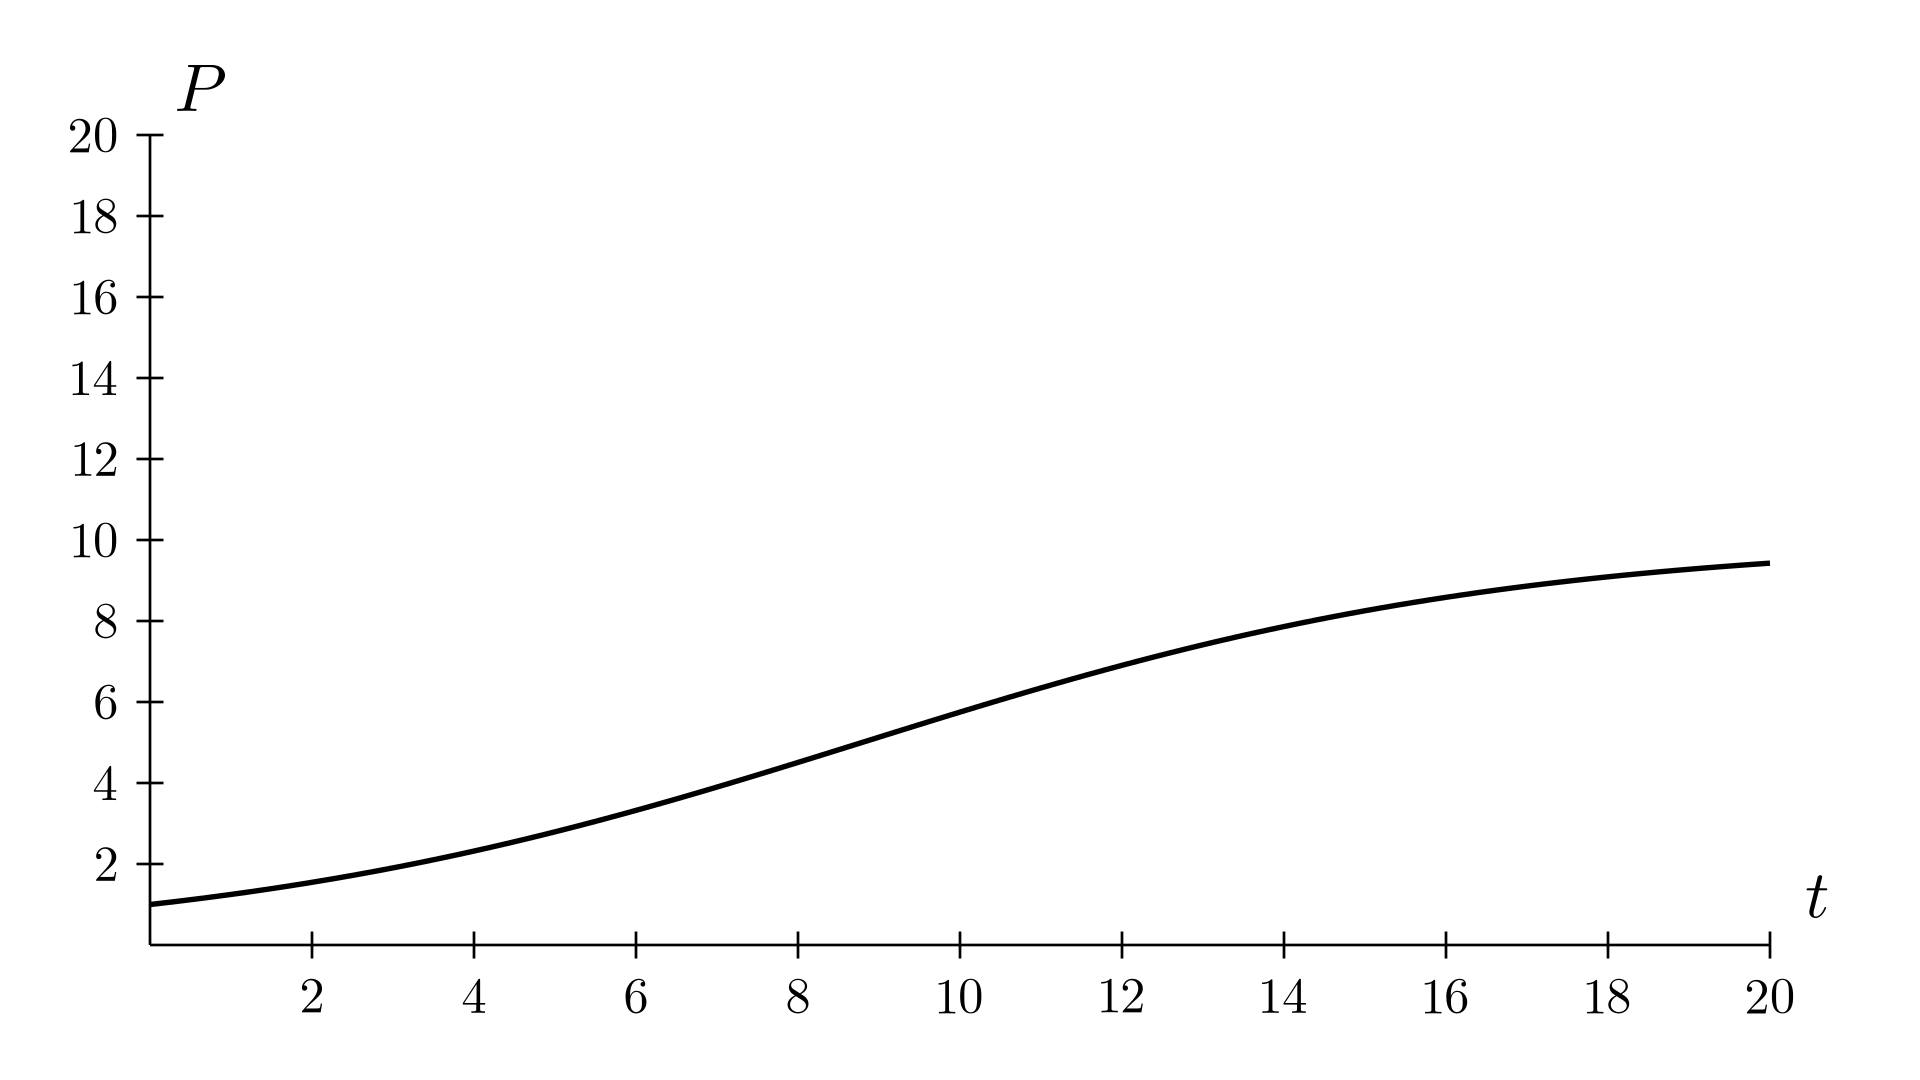
\includegraphics[width=10cm]{LogisticSingle}
\end{center}
% P = lambda t : -(2*math.e**(k * t + c))/( 1 - math.e**(k * t + c) )

Here, we can see our solution approaches a certain value, the equillibria, in the graph and slows down its growth or decay. When we are above this line, we see our solution is always decaying. When we are below this line, we see our solution is always growing. Eventually, the growth and decay slows down to a halt.

What does this graph tell us? Looking at this graph, we can predict the growth or decay of our rabbit population. If we pick a point underneath the equillibria, then we should expect our population to grow until our population reaches the threshold. If we pick a point above this line, we should expect our population to decay until we reach the threshold.

\begin{center}
  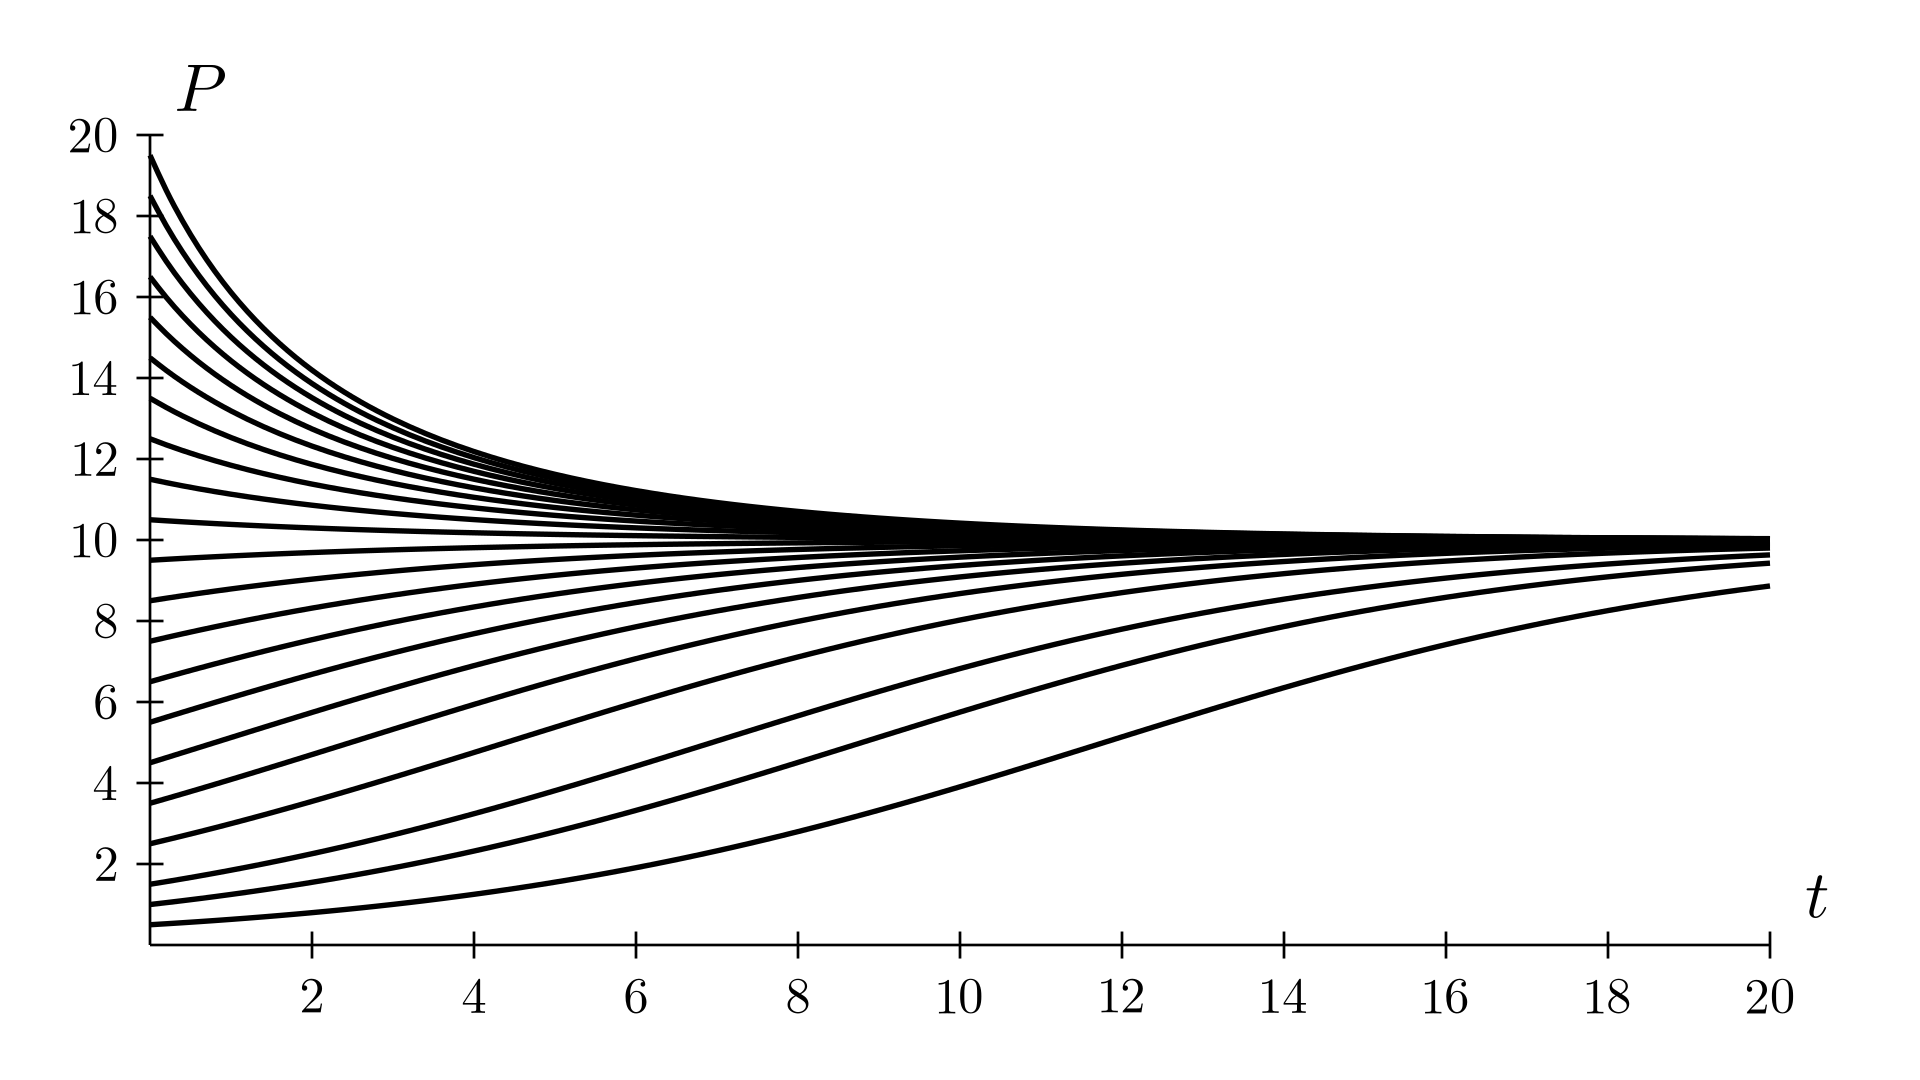
\includegraphics[width=10cm]{LogisticGroup}
\end{center}
% Produce the graph.

\section{Predator-Prey Sytems}

Now, let us modify our model one more time. We created a logistic population model for the rabbits in our forest. However, we only took account for limited resources in a given area. In the real world, the rabbit population also depends on how many predators are in the area. If there are a lot of predators in the area, then the rabbit population might shrink until foxes can no longer find rabbits with ease. Let us consider a model with the following parameters:
\begin{enumerate}
  \item R: Rabbit Population
  \item $\alpha$: Growth-rate for Rabbits
  \item $\beta$: Death-rate between Rabbits-Foxes interaction.
  \item F: Fox Population
\end{enumerate}

Taking a look at our scenario and parameters, we can find the following model:

\begin{align*}
  \frac{dR}{dt} & = \alpha R - \beta RF
\end{align*}

Here, $\alpha$ and $\beta$ are constant values. We can see as the fox population increases, more rabits are hunted and removed from the population. However, note that $F$ is a variable similar as $R$. If we can model $R$, how might we model $F$?

Since we know foxes benefit from interacting with rabbits, what would happen if all the rabbits disappeared from the area? Those foxes depend on rabbits to sustain their population. Without rabbits, we can expect the fox population to decline at a given rate. Let us consider a few more parameters:
\newpage
\begin{enumerate}
  \item F: Fox Population
  \item $\gamma$: Decay-rate for Foxes
  \item $\delta$: Beneficial-rate for Fox-Rabbit interactions.
  \item R: Rabbit Population
\end{enumerate}

Here, let us take a look at our model for the Rabbit population and our new model for the Fox population:

\begin{align*}
  \frac{dR}{dt} & = \alpha R - \beta RF\\
  \frac{dF}{dt} & = -\gamma F + \delta FR
\end{align*}

Here, we can see a relationship between the Rabbit population and the Fox population. This first-order system have variables which depend on each other. The size of the Rabbit population is dependent on the size of the Fox population and vice versa.
% Note that when the Fox population is empty, or $F = 0$, then the Rabbit population can be written as:
%\begin{align}
%  \frac{dR}{dt} & = \alpha R
%\end{align}
Let us take a look at what our graph looks like when $\alpha = 2$, $\beta = 1.6$, $\gamma = 1$, and $\delta = 0.8$

\begin{center}
  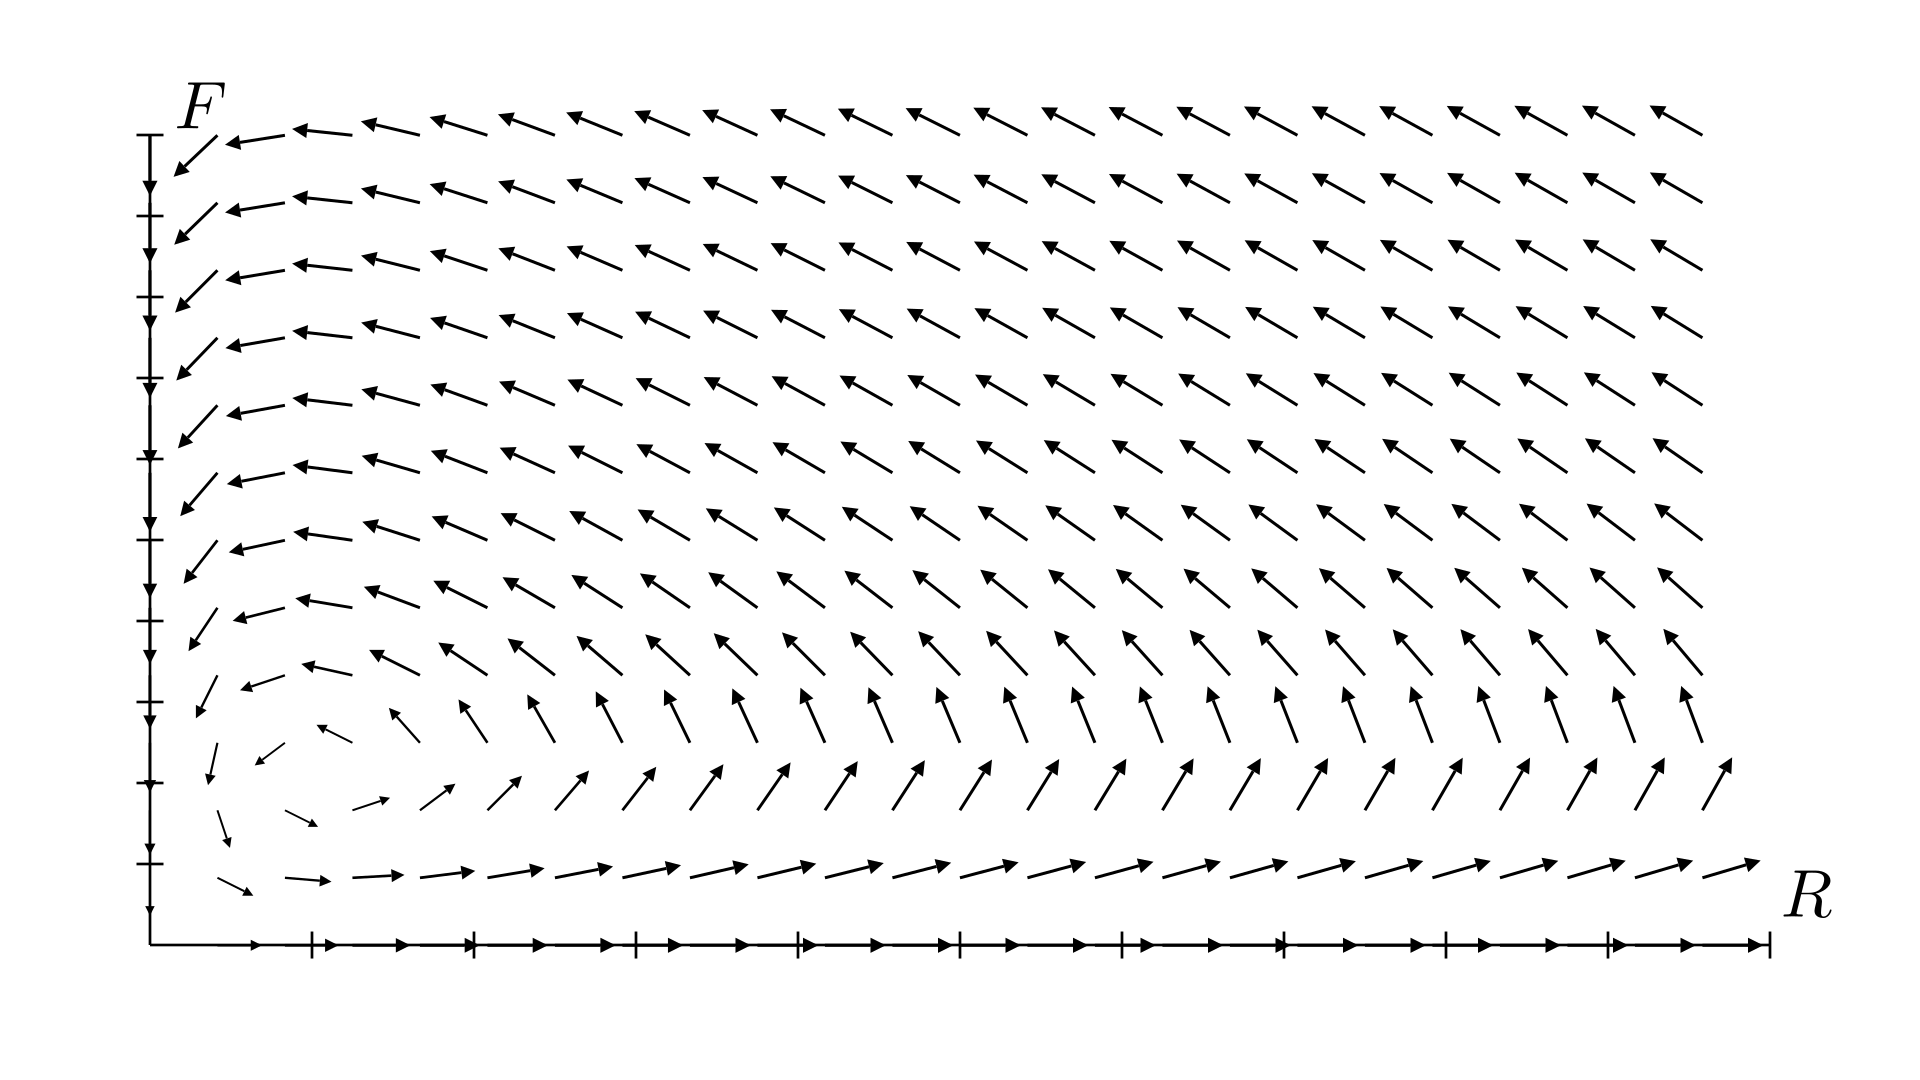
\includegraphics[width=10cm]{PredatorPreyModel}
\end{center}

% Graph here

Looking at our graph, we can see our Rabbit population and Fox population dance around a point in the graph. Here, the graph is moving about the system's equilibrium point. Let us take a look at how $R$ and $F$ grow and decay as time goes on in a $R-t$ and $F-t$ graph:

\[ Graph Here \]
% Rt graph, Ft graph, both together at once

Here, we can see there are times when our Rabbit population will grow until the population hits a peak and begin to shrink again, repeating the process over again. The Fox population exhibits a similar graph. However, when we stack both graphs ontop of each other, we can see the peak for the Fox population occurs right after the Rabbit population peak. In addition, we can see as the Fox population decreases, the Rabbit population benefits and begins to grow once more.


\section{SIR Modeling}

How can we configure our Predator-Prey model to model an epidemic? Here, let us consider the stages of an infection, such as the common cold. At first, we might consider a healthy individual who is not infected. Once the individual catches the infection, the individual might go a few days with the illness. However, after a few more days, the individual will recover and potentially have a stronger immune system to combat against that infection.

Here, we can see we go through three phases: susceptible, infected, and recovered phases. Also note that when we expand this model to a community, we might consider a fraction of the population to be susceptible, infected, or recovered. For this model, we consider and deceased individuals as recovered Here, we have a few variables we are considering:

\begin{enumerate}
  \item $s(t) = S$: Number of susceptible individuals
  \item $i(t) = I$: Number of infected individuals
  \item $r(t) = R$: Number of recovered individuals
\end{enumerate}

Now, how might we model our pandemic? Let us consider our susceptible population. Our susceptible population is decreasing at a rate proportional to the interaction between susceptible and infected individuals. Our infected population increases by the same interaction. In addition, our infected population decreases at a rate proportional to the recovery rate. Our recovered population increases by the same rate. With our given assumptions, we can create the following model where $\alpha$ is the infection rate and $\beta$ is the recovery rate:
% Refractor SIR to sir? -- hey, those were my old initials!
\begin{align*}
  \dS & = -\alpha SI\\
  \dI & = \alpha SI - \beta I\\
  \dR & = \beta I
\end{align*}

Consider our population, $N$. Here, $N$ can represent the population of the globe or the population of one's community. If we look at our population, note that the population size is constant throughout the model. In the predator-prey model, the population size fluctuates as we move forward in time. In our SIR model, our size is constant. This means we can rewrite our variables as:
%
\begin{enumerate}
  \item $s(t)/N = S(t)$: Percentage of population considered as Susceptible
  \item $i(t)/N = I(t)$: Percentage of population considered as Infected
  \item $r(t)/N = R(t)$: Percentage of population considered as Recovered
\end{enumerate}

Here, since $S(t)$, $I(t)$, and $R(t)$ are all a fraction of our population. If we add them all together, we should find $S(t) + I(t) + R(t) = 1$

\section{Visualizing our Pandemic}

Let us put a pin on our differential equations and let us visualize portions of our model to help understand why each component is important.

First, let us consider how fast an infection can spread starting from one individual. Let us assume all infected individuals remain infected and each infected individual infects one non-infected individual at each time step.

\[ Model here \]
% 1 infected to 1 -> 2
% 2 infected to 2 -> 4
% 4 infected to 4 -> 8

Looking at our model, we can see our number of infected individuals double after every time interval. If the time step is one day, that means we will have a population of 16 infected individuals after 4 days. What would happen if we let this simulation run for more days? How long would it take to infect our entire population? If we let our population be $100000$, how long would it take to infect everyone starting from one infected individual?

\[ Graph Here \]
% aI %

The growth at the start of our graph starts out slow. It takes time for the infection to catch wind and start spreading fast throughout the population. Fortunately for us, infections cannot exhibit such exponential growth. Consider this: If the population is roughly $100\%$ susceptible, then the individuals that the infected person comes into contact with is roughly $100\%$. If $50\%$ of the population is susceptible, then the infected should expect its contacted people to be about $50\%$ susceptible. Here, let us visualize the infected person's interactions:

\[ Image here \]
% 1 to 10 | 1 to 5/5 | 1 to 0/10

Here, recall we modified our first population model and created a logistic population model. Let us see how a logistic growth can change the way our model runs:

\[ Graph here \]
% Logistic Growth Curve

Here, our graph exhibits a slow growth at the start, a rapid growth when our population is roughly $50\%$ infected, then a slow growth as our infected population reaches $100\%$.

Now, we know when we become infected, we can recover from the infection. Now, let us make the assumption that once an individual recovers from an infection, the individual becomes immune to the infection. Let us consider a population made up of $100\%$ infected individuals. If infected individuals become recovered at a rate of $\beta$. Here is what our graph looks like when our population can recover from the infection:

\[ Graph here \]
% Exponential decay curve

How would our graph look like if we let our population become infected and recover from the infection?

\[ Graph here \]
% SIR Model

This graph represents our SIR model. Other SIR models consider many more factors, such as increasing population, vaccinations rates, mask rates, and so on.

Why might our infection grow? In epidemiology, diseases are  associated with a reproduction number. This reproduction number is the average number of people an infected individual can infect before the infected individual can recover. As an outbreak ensues, the infection's reproduction number, R, changes. When an infection begins, the infection's initial $R$ is considered $R_0$. What might $R$ look like if $R_0$ is greater than $1$?

\[ Images here \]
% R_0 > 1 | R = 1 | R < 1

% -- 1 -- https://www.news-medical.net/health/What-is-R0.aspx %
To give a perspective, the common cold has an $R_0$ of about $2-3$ and Measles has an $R_0$ of $12-18$.

How might we start looking for $R_0$? To begin, we can look at how many days it would take for an infected individual to infect one person. In addition, we may look at how long it will take for an infected person to recover. For example, if a person infects one person every four days and it takes the infected individual eight days to recover, we can expect $R_0$ to be $2$. However, if it takes two days to recover, then $R_0$ would be $0.5$.

% -- 2 -- https://www.cdc.gov/coronavirus/2019-ncov/php/contact-tracing/contact-tracing-plan/prioritization/mathematicalmodeling.html %
If we can make $R < 1$, then we have reached herd immunity. We can lower $R$ through measures such as quarantining, contact tracing, and vaccine campaigns.

\newpage

And finally, the references you used (if any):

\bibliographystyle{plain}
\begin{thebibliography}{12}

\bibitem{milnor}
John Milnor, {\it
 American Mathematical Monthly}
    {\bf 85} (7), August-September 1978, 521--528.

 \smallskip

    \bibitem{alexandrov}
    P.~S.~Aleksandrov, {\it Combinatorial Topology},
    Dover Publications, 1998.


\end{thebibliography}

% --1-- https://www.news-medical.net/health/What-is-R0.aspx

\newpage
\section{Paul's Online Notes}
https://tutorial.math.lamar.edu/Classes/DE/DE.aspx\\
\lipsum[0-2]

\section{Differential Equations by Paul Blanchard, Robert Devaney, Glen Hall}
\underline{Unlimited Growth}\\ % 4
\lipsum[2-4]\\
\underline{Logistic Population Models}\\ % 9
\lipsum[4-6]\\
\underline{Predator-Prey System}\\ % 12, 150
\lipsum[6-8]\\
\underline{The SIR Model of an epidemic}\\ % 210
\lipsum[8-10]

\section{The SIR Model for Spread of Disease}
https://www.maa.org/press/periodicals/loci/joma/the-sir-model-for-spread-of-disease-the-differential-equation-model\\
\lipsum[0-2]

\section{COVID-19 Futures, Explained with Simulations}
https://ncase.me/covid-19/\\
\lipsum[3-5]

\section{How Outbreaks Like Coronavirus Spread Exponentially, and How To "Flatten the Curve"}
https://www.washingtonpost.com/graphics/2020/world/corona-simulator/\\
\lipsum[1-3]

\section{Modeling Exponential Growth}
https://www.youtube.com/watch?v=Kas0tIxDvrg\\
\lipsum[2-3]

\section{Modeling COVID-19 with Differential Equations}
% https://julia.quantecon.org/continuous_time/seir_model.html \\
\lipsum[3-4]
\end{sansmath}



\end{document}
